{\bf This problem was reconstructed to fullfill the interactive problem environment. It differs from the judging system that was available on IOI. }

We consider a two-player game. The players are given an $x \times y$ rectangle (where $x$ and $y$ are positive integers).
The players take turns moving. A move consists of dividing a rectangle into two rectangles with a single
vertical or horizontal cut. The resulting rectangles must have positive integer dimensions.

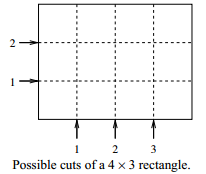
\includegraphics{rectangle.png}

After each cut, the smaller rectangle (that is the one with smaller area) is discarded and the other one is passed
to the other player. If the rectangle is cut into two equal halves, then one half is discarded. The player who
receives a $1 \times 1$ rectangle, and therefore is not able to make a move, loses the game.

Your task is to write a program to play and win the rectangle game. 
Initial rectangle sizes are from  $1$ to $100\,000\,000$. At least on of them is greater than 1. 
